\documentclass[11pt,a4paper]{article}

\usepackage[T1]{fontenc}
\usepackage[utf8]{inputenc}
\usepackage{lmodern}
\usepackage{microtype}
\usepackage[margin=2.3cm]{geometry}
\usepackage{amsmath,amssymb}
\usepackage{graphicx}
\usepackage{booktabs}
\usepackage{longtable}
\usepackage{array}
\usepackage[font=small,labelfont=bf]{caption}
\usepackage{xcolor}
\usepackage{fancyvrb}
\usepackage{enumitem}
\usepackage[numbers,sort&compress]{natbib}
\usepackage{url}
\def\UrlBreaks{\do\_\do\-\do\.\do\/}
\usepackage[colorlinks=true,linkcolor=blue!50!black,citecolor=blue!50!black,urlcolor=blue!50!black]{hyperref}

\setlength{\parskip}{0.35em}
\setlist{itemsep=0.15em,topsep=0.3em}
\graphicspath{{figures/}}
\newcommand{\spNord}{49}
\newcommand{\spNpix}{4088}
\newcommand{\spMfirst}{79}
\newcommand{\spMlast}{31}
\newcommand{\spWmin}{964.6}
\newcommand{\spWmax}{2490.2}
\newcommand{\spLref}{1496.2}
\newcommand{\spTeff}{5000}
\newcommand{\spNtotal}{200\,312}
\newcommand{\spNvalid}{163\,678}
\newcommand{\spValidPct}{81.7}
\newcommand{\spNfitted}{163\,678}
\newcommand{\spNuse}{162\,735}
\newcommand{\spNlike}{10\,165}
\newcommand{\spNwin}{4\,947}
\newcommand{\spDec}{16}
\newcommand{\spCorr}{601}
\newcommand{\spNeff}{271}
\newcommand{\spNu}{1.73}
\newcommand{\spTscale}{1.06}
\newcommand{\spMad}{1.33}
\newcommand{\spResStd}{2.61}
\newcommand{\spKurt}{13.4}
\newcommand{\spSkew}{-1.61}
\newcommand{\spTemper}{1/38}
\newcommand{\spBestCzero}{76798.1}
\newcommand{\spBestCone}{-0.1147}
\newcommand{\spBestBeta}{0.8556}
\newcommand{\spBestAsym}{-3.432}
\newcommand{\spBestAzero}{76969.79}
\newcommand{\spBestAone}{-0.11474}
\newcommand{\spBestChange}{-0.228}
\newcommand{\spCzero}{76802.0^{+1.4}_{-1.4}}
\newcommand{\spCone}{-0.1070^{+0.0026}_{-0.0026}}
\newcommand{\spBeta}{0.85596^{+0.00078}_{-0.00073}}
\newcommand{\spAsym}{-3.45^{+0.20}_{-0.19}}
\newcommand{\spLns}{-4.668^{+0.081}_{-0.078}}
\newcommand{\spAzero}{76962.0^{+3.4}_{-3.3}}
\newcommand{\spAone}{-0.1070^{+0.0026}_{-0.0026}}
\newcommand{\spDlnc}{-2.084^{+0.050}_{-0.050}}
\newcommand{\spChange}{-0.2125^{+0.0051}_{-0.0051}}
\newcommand{\spChangeVal}{-0.212}
\newcommand{\spChangeAbs}{0.212}
\newcommand{\spChangeSig}{41}
\newcommand{\spChangeSigJack}{24}
\newcommand{\spSigCzero}{1.4}
\newcommand{\spJackCzero}{2.2}
\newcommand{\spRatioCzero}{1.5}
\newcommand{\spSigCone}{0.0026}
\newcommand{\spJackCone}{0.0044}
\newcommand{\spRatioCone}{1.7}
\newcommand{\spSigBeta}{0.00075}
\newcommand{\spJackBeta}{0.00110}
\newcommand{\spRatioBeta}{1.5}
\newcommand{\spSigAsym}{0.19}
\newcommand{\spJackAsym}{0.32}
\newcommand{\spRatioAsym}{1.7}
\newcommand{\spSigAzero}{3.3}
\newcommand{\spJackAzero}{6.4}
\newcommand{\spSigAone}{0.0026}
\newcommand{\spJackAone}{0.0044}
\newcommand{\spSigChange}{0.0051}
\newcommand{\spJackChange}{0.0088}
\newcommand{\spSigDlnc}{0.050}
\newcommand{\spJackDlnc}{0.086}
\newcommand{\spCorrCzeroCone}{0.53}
\newcommand{\spCorrBetaAsym}{0.05}
\newcommand{\spCorrCzeroAsym}{0.85}
\newcommand{\spCorrConeAsym}{0.25}
\newcommand{\spMaxCorr}{0.85}
\newcommand{\spCorrPair}{$c_0$ and $\alpha$}
\newcommand{\spCorrPairVal}{0.85}
\newcommand{\spTauMax}{57}
\newcommand{\spTauMin}{51}
\newcommand{\spNsteps}{12\,000}
\newcommand{\spStepsOverTau}{211}
\newcommand{\spBurn}{170}
\newcommand{\spThin}{25}
\newcommand{\spNsamples}{15\,136}
\newcommand{\spAcc}{0.55}
\newcommand{\spNwalkers}{32}
\newcommand{\spDlpConst}{268}
\newcommand{\spConstCzero}{76842.5}
\newcommand{\spDlpLittrow}{134}
\newcommand{\spAsymLittrow}{1.00}
\newcommand{\spTeffDlpMid}{0.15}
\newcommand{\spTeffDlpMax}{0.23}
\newcommand{\spTeffShift}{0.121}
\newcommand{\spLittrowSig}{22.4}
\newcommand{\spLittrowSigJack}{13.7}
\newcommand{\spDlpLittrowDec}{134.5}
\newcommand{\spPkMapMean}{-2}
\newcommand{\spPkMapRms}{19}
\newcommand{\spPkConstMean}{-46}
\newcommand{\spPkConstRms}{43}
\newcommand{\spMedRel}{0.76}
\newcommand{\spRmsRel}{4.36}
\newcommand{\spMedPerOrder}{1.74}
\newcommand{\spPerOrderQlo}{0.98}
\newcommand{\spPerOrderQhi}{2.45}
\newcommand{\spWorst}{31 (21\%), 35 (5\%), 78 (5\%)}
\newcommand{\spScatBest}{1.78\times10^{-3}}
\newcommand{\spScatSecond}{3.98\times10^{-3}}
\newcommand{\spScatRatio}{2.2}
\newcommand{\spRunnerUp}{80}
\newcommand{\spMlamMean}{76742.3}
\newcommand{\spGradStart}{79}
\newcommand{\spScatCBest}{3.4\times10^{-4}}
\newcommand{\spScatCRatio}{15}
\newcommand{\spOverlapMaxDev}{0.27}
\newcommand{\spGradMaxDev}{0.27}
\newcommand{\spGradEdgeFirst}{-1.27}
\newcommand{\spGradEdgeLast}{+0.98}
\newcommand{\spOverlapMeanDev}{-0.09}
\newcommand{\spExtLin}{26}
\newcommand{\spExtCub}{18}
\newcommand{\spExtPoly}{2\times10^{7}}
\newcommand{\spChangeRangeLo}{-0.236}
\newcommand{\spChangeRangeHi}{-0.228}
\newcommand{\spCubDiffMed}{0.02}
\newcommand{\spFitMed}{0.90}
\newcommand{\spFitRms}{4.26}
\newcommand{\spFitPerOrder}{1.64}
\newcommand{\spFitWorst}{31 (21\%), 78 (5\%), 35 (5\%)}
\newcommand{\spPeakDrift}{803}
\newcommand{\spPkConstMax}{154}
\newcommand{\spPkConstMaxOrder}{38}
\newcommand{\spPkMapFirst}{-49}
\newcommand{\spPkMapMaxPos}{33}
\newcommand{\spPkMapMaxPosOrder}{45}
\newcommand{\spLikeCheck}{6\times10^{-8}}
\newcommand{\spKnotCheck}{10^{-14}}
\newcommand{\spLikeMs}{0.4}
\newcommand{\spDwaveVar}{28}
\newcommand{\spTransRange}{32}
\newcommand{\spMedRatioConst}{2.6}
\newcommand{\spTwoDsin}{77105.8}
\newcommand{\spCblue}{76858.8}
\newcommand{\spCred}{76695.6}
\newcommand{\spGammaBlue}{4.59}
\newcommand{\spGammaRed}{5.91}
\newcommand{\spGammaDelta}{1.33}
\newcommand{\spGrooves}{23.2}
\newcommand{\spCdrop}{163}
\newcommand{\niNord}{75}
\newcommand{\niNpix}{4088}
\newcommand{\niMfirst}{149}
\newcommand{\niMlast}{75}
\newcommand{\niWmin}{969.0}
\newcommand{\niWmax}{1954.0}
\newcommand{\niLref}{1336.1}
\newcommand{\niTeff}{5000}
\newcommand{\niNtotal}{306\,600}
\newcommand{\niNvalid}{260\,904}
\newcommand{\niValidPct}{85.1}
\newcommand{\niNfitted}{260\,904}
\newcommand{\niNuse}{257\,850}
\newcommand{\niNlike}{16\,110}
\newcommand{\niNwin}{7\,549}
\newcommand{\niDec}{16}
\newcommand{\niCorr}{833}
\newcommand{\niNeff}{310}
\newcommand{\niNu}{1.01}
\newcommand{\niTscale}{1.13}
\newcommand{\niMad}{1.72}
\newcommand{\niResStd}{10.00}
\newcommand{\niKurt}{32.4}
\newcommand{\niSkew}{0.28}
\newcommand{\niTemper}{1/52}
\newcommand{\niBestCzero}{145020.5}
\newcommand{\niBestCone}{-0.0811}
\newcommand{\niBestBeta}{0.8586}
\newcommand{\niBestAsym}{3.495}
\newcommand{\niBestAzero}{145128.85}
\newcommand{\niBestAone}{-0.08111}
\newcommand{\niBestChange}{-0.055}
\newcommand{\niCzero}{145026.0^{+1.7}_{-1.6}}
\newcommand{\niCone}{-0.0748^{+0.0043}_{-0.0042}}
\newcommand{\niBeta}{0.8584^{+0.0014}_{-0.0014}}
\newcommand{\niAsym}{5.51^{+0.60}_{-0.60}}
\newcommand{\niLns}{-4.536^{+0.085}_{-0.083}}
\newcommand{\niAzero}{145125.9^{+5.1}_{-5.1}}
\newcommand{\niAone}{-0.0748^{+0.0043}_{-0.0042}}
\newcommand{\niDlnc}{-0.689^{+0.039}_{-0.039}}
\newcommand{\niChange}{-0.0508^{+0.0029}_{-0.0029}}
\newcommand{\niChangeVal}{-0.051}
\newcommand{\niChangeAbs}{0.051}
\newcommand{\niChangeSig}{18}
\newcommand{\niChangeSigJack}{13}
\newcommand{\niSigCzero}{1.7}
\newcommand{\niJackCzero}{2.3}
\newcommand{\niRatioCzero}{1.4}
\newcommand{\niSigCone}{0.0043}
\newcommand{\niJackCone}{0.0058}
\newcommand{\niRatioCone}{1.4}
\newcommand{\niSigBeta}{0.0014}
\newcommand{\niJackBeta}{0.0032}
\newcommand{\niRatioBeta}{2.3}
\newcommand{\niSigAsym}{0.60}
\newcommand{\niJackAsym}{0.89}
\newcommand{\niRatioAsym}{1.5}
\newcommand{\niSigAzero}{5.1}
\newcommand{\niJackAzero}{6.8}
\newcommand{\niSigAone}{0.0043}
\newcommand{\niJackAone}{0.0058}
\newcommand{\niSigChange}{0.0029}
\newcommand{\niJackChange}{0.0039}
\newcommand{\niSigDlnc}{0.039}
\newcommand{\niJackDlnc}{0.053}
\newcommand{\niCorrCzeroCone}{0.47}
\newcommand{\niCorrBetaAsym}{0.59}
\newcommand{\niCorrCzeroAsym}{0.81}
\newcommand{\niCorrConeAsym}{0.16}
\newcommand{\niMaxCorr}{0.81}
\newcommand{\niCorrPair}{$c_0$ and $\alpha$}
\newcommand{\niCorrPairVal}{0.81}
\newcommand{\niTauMax}{63}
\newcommand{\niTauMin}{58}
\newcommand{\niNsteps}{16\,000}
\newcommand{\niStepsOverTau}{255}
\newcommand{\niBurn}{188}
\newcommand{\niThin}{28}
\newcommand{\niNsamples}{18\,048}
\newcommand{\niAcc}{0.55}
\newcommand{\niNwalkers}{32}
\newcommand{\niDlpConst}{100}
\newcommand{\niConstCzero}{145039.3}
\newcommand{\niDlpLittrow}{3}
\newcommand{\niAsymLittrow}{7.00}
\newcommand{\niTeffDlpMid}{0.02}
\newcommand{\niTeffDlpMax}{0.03}
\newcommand{\niTeffShift}{0.030}
\newcommand{\niLittrowSig}{2.5}
\newcommand{\niLittrowSigJack}{1.7}
\newcommand{\niDlpLittrowDec}{3.2}
\newcommand{\niPkMapMean}{15}
\newcommand{\niPkMapRms}{292}
\newcommand{\niPkConstMean}{-6}
\newcommand{\niPkConstRms}{266}
\newcommand{\niMedRel}{1.11}
\newcommand{\niRmsRel}{28.49}
\newcommand{\niMedPerOrder}{2.03}
\newcommand{\niPerOrderQlo}{1.19}
\newcommand{\niPerOrderQhi}{2.76}
\newcommand{\niWorst}{78 (166\%), 75 (87\%), 104 (36\%)}
\newcommand{\niScatBest}{1.21\times10^{-3}}
\newcommand{\niScatSecond}{2.15\times10^{-3}}
\newcommand{\niScatRatio}{1.8}
\newcommand{\niRunnerUp}{150}
\newcommand{\niMlamMean}{144963.1}
\newcommand{\niGradStart}{149}
\newcommand{\niScatCBest}{8.0\times10^{-4}}
\newcommand{\niScatCRatio}{2}
\newcommand{\niOverlapMaxDev}{44.94}
\newcommand{\niGradMaxDev}{12.61}
\newcommand{\niGradEdgeFirst}{-1.04}
\newcommand{\niGradEdgeLast}{-8.44}
\newcommand{\niOverlapMeanDev}{-0.11}
\newcommand{\niChangeRangeLo}{-0.056}
\newcommand{\niChangeRangeHi}{-0.046}
\newcommand{\niCubDiffMed}{0.01}
\newcommand{\niFitMed}{1.20}
\newcommand{\niFitRms}{26.35}
\newcommand{\niFitPerOrder}{1.85}
\newcommand{\niFitWorst}{78 (151\%), 75 (81\%), 104 (36\%)}
\newcommand{\niPeakDrift}{1628}
\newcommand{\niPkConstMax}{1241}
\newcommand{\niPkConstMaxOrder}{105}
\newcommand{\niPkMapFirst}{6}
\newcommand{\niPkMapMaxPos}{1146}
\newcommand{\niPkMapMaxPosOrder}{75}
\newcommand{\niLikeCheck}{6\times10^{-8}}
\newcommand{\niKnotCheck}{10^{-15}}
\newcommand{\niLikeMs}{0.7}
\newcommand{\niDwaveVar}{56}
\newcommand{\niTransRange}{33}
\newcommand{\niMedRatioConst}{1.4}
\newcommand{\MaxRatio}{2.3}
\newcommand{\MinRatio}{1.4}
\newcommand{\ChangeRatio}{4.2}
\newcommand{\ExpAccA}{1.5\times10^{-4}}
\newcommand{\ExpAccB}{1.3\times10^{-3}}
\newcommand{\ExpAccC}{3.0\times10^{-2}}
\newcommand{\PeakRatio}{1.27}


\newcommand{\lamb}{\lambda_{\rm b}}
\newcommand{\sinc}{\operatorname{sinc}}
\newcommand{\code}[1]{\texttt{#1}}
\newcommand{\apero}{\textsc{apero}}
% table rows read from a file: the primitive input, because \input inside a
% tabular breaks a following \midrule
\makeatletter
\newcommand{\rows}[1]{\@@input #1 }
\makeatother

\title{A physical model of the \'echelle blaze function\\[0.3em]
\large Order identification, a chromatic grating constant, and an MCMC characterisation on SPIRou and NIRPS flat fields}
\author{\'Etienne Artigau}
\date{\today}

\begin{document}
\maketitle

\begin{abstract}
We model the blaze of an \'echelle spectrograph, as measured on a flat-lamp exposure, as the product of four physical terms: the photon spectrum of the lamp, the transmission of the instrument, the diffraction envelope of a single grating groove, and the wavelength width of a pixel. The diffraction order of every spectral order is first recovered from the wavelength solution alone, with two independent methods that agree without ambiguity: SPIRou covers orders \spMfirst\ to \spMlast\ and NIRPS orders \niMfirst\ to \niMlast. The grating constant $C = m\lamb$ is found to be chromatic. Letting it vary linearly with wavelength divides the median residual of the SPIRou fit by \spMedRatioConst\ and removes a systematic offset of up to \spPkConstMax\ pixels between the observed and modelled order peaks. The effect is expected from SPIRou's cross-disperser, which the beam crosses before reaching the grating. $C$ changes by $\spChange\%$ across SPIRou and $\niChange\%$ across NIRPS. An MCMC, built on a likelihood that accounts for the strongly correlated, heavy-tailed residuals, gives the posterior of the grating parameters. A jackknife over orders gives uncertainties \MinRatio\ to \MaxRatio\ times larger, which is the level at which the error bars should be trusted. The model reproduces the SPIRou blaze to a median of \spMedRel\% per pixel and is defined on every pixel, including those the pipeline discards.
\end{abstract}

\tableofcontents

%======================================================================
\section{Introduction}

The blaze function of an \'echelle spectrograph describes how efficiently each order delivers light as a function of wavelength. Reduction pipelines such as \apero\ \citep{Cook2022} measure it empirically on a flat-lamp exposure, smooth it, and discard it where it falls below a threshold. That is sufficient to flat-field the science data, but it says nothing about \emph{why} the blaze has the shape it has, and it leaves the edges of every order undefined.

This report builds the blaze from the physics that produces it, fits the handful of free parameters to a flat-lamp exposure, and characterises their uncertainties. The approach is instrument-agnostic, since nothing in the code knows which spectrograph it is looking at. It is applied here to SPIRou \citep{Donati2020} and, as an independent check, to NIRPS \citep{Artigau2024}. All numbers quoted in the text are written by the analysis scripts themselves (Appendix~\ref{app:repro}), apart from one exploratory test, which is marked as such.

%======================================================================
\section{Data}
\label{sec:data}

For each instrument, the analysis uses two \apero\ products, both $N_{\rm ord}\times N_{\rm pix}$ arrays.
\begin{itemize}
\item The \emph{blaze}: the extracted flat-lamp spectrum. For SPIRou it is \path{FDFCD50E5Ff_pp_blaze_AB.fits}, and for NIRPS \path{NIRPS_2023-04-01T12_07_06_942_pp_blaze_A.fits}. \apero\ sets it to NaN wherever it falls below 25\% of the order maximum, so only the top of each order is available.
\item The \emph{wavelength solution}, the wavelength of every pixel. For SPIRou it is \path{FEF450D367a_pp_e2dsff_AB_wave_night_AB.fits}, and for NIRPS \path{NIRPS_2025-09-13T21_30_32_350_pp_e2dsff_A_wave_night_A.fits}.
\end{itemize}

SPIRou provides $\spNord\times\spNpix$ pixels ($\spNtotal$ in total, $\spValidPct\%$ with a valid blaze) from \spWmin\ to \spWmax~nm. NIRPS provides $\niNord\times\niNpix$ ($\niValidPct\%$ valid) from \niWmin\ to \niWmax~nm, with a gap between the J and H bands. The NIRPS blaze (2023) and wavelength solution (2025) were taken two years apart. The fit is good regardless, but a drift of the wavelength solution between the two dates cannot be excluded.

%======================================================================
\section{Identifying the diffraction orders}
\label{sec:orders}

Extracted spectra are indexed by their position in the file, $k = 0\dots N_{\rm ord}-1$, not by their diffraction order $m$. The model needs $m$. Two independent methods recover it from the data. Both are implemented in \code{mkblaze.py}, and \code{fit\_blaze.py} uses a variant of each.

\subsection{Flatness of $m\lambda$ at the blaze peak}

Every order is blazed by the same grooves, so the wavelength of the blaze maximum obeys $m_k\lambda_{{\rm b},k} = C$ for all $k$. When orders are stored from blue to red, $m_k = m_0 - k$ for an unknown integer $m_0$. \code{mkblaze.py} takes the wavelength of the maximum of the observed blaze, $\lambda^{\rm peak}_k$, and scans $m_0$:
\begin{equation}
S(m_0) = \frac{\sigma\left[(m_0-k)\,\lambda^{\rm peak}_k\right]}{\left\langle (m_0-k)\,\lambda^{\rm peak}_k\right\rangle},
\qquad m_0 \in [N_{\rm ord}+1,\,200).
\label{eq:scatter}
\end{equation}
For SPIRou the minimum is at $m_0 = \spMfirst$, with $S = \spScatBest$. The runner-up, $m_0=\spRunnerUp$, gives $\spScatSecond$, which is \spScatRatio\ times worse. The mean of $m\lambda^{\rm peak}$ is \spMlamMean~nm. For NIRPS, $m_0=\niMfirst$ with $S=\niScatBest$, \niScatRatio\ times better than $m_0 = \niRunnerUp$.

\code{fit\_blaze.py} applies the same criterion to the wavelength of the central pixel, $\lambda^{\rm c}_k$, instead of the blaze maximum. This is justified in the next subsection. It is sharper, because it does not depend on where the lamp spectrum places each maximum: the best $m_0$ gives $S = \spScatCBest$ for SPIRou, \spScatCRatio\ times lower than the next integer (Figure~\ref{fig:orderscan}).

\begin{figure}[t]
\centering
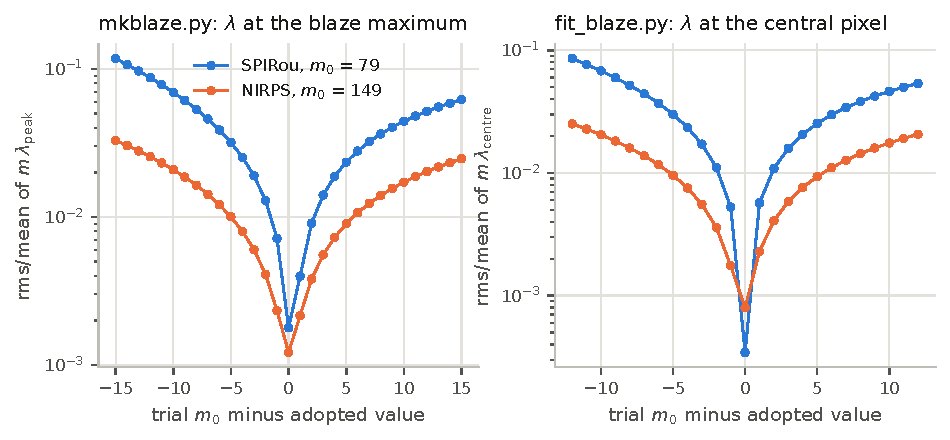
\includegraphics[width=\textwidth]{orders_scan.pdf}
\caption{Relative scatter of $m\lambda$ across orders against the trial first order, for SPIRou and NIRPS. Left: at the wavelength of the blaze maximum (\code{mkblaze.py}). Right: at the central pixel (\code{fit\_blaze.py}). The minimum is unambiguous in both cases.}
\label{fig:orderscan}
\end{figure}

\subsection{Overlap of consecutive orders}

At a given pixel $x$, all orders are diffracted at the same angle, so the grating equation gives $m_k\lambda_k(x) = m_{k+1}\lambda_{k+1}(x)$. With $m_{k+1}=m_k-1$,
\begin{equation}
m_k = \frac{\lambda_{k+1}(x)}{\lambda_{k+1}(x)-\lambda_k(x)}.
\label{eq:overlap}
\end{equation}
This estimate needs only the wavelength solution, not the blaze. \code{mkblaze.py} evaluates it at the central pixel. For the last order, which has no successor, the estimate is taken as that of the previous order minus one. The continuous version, $m = \lambda/|d\lambda/dk|$, where $d\lambda/dk$ is a central difference across orders, does not depend on the storage direction. It is the one \code{fit\_blaze.py} uses to obtain a starting value ($m_0 = \spGradStart$ for SPIRou) before the flatness scan.

Neither estimator is exactly an integer, because $m\lambda$ is not exactly constant at a fixed pixel. For SPIRou, the overlap estimate deviates from the adopted $m$ by at most \spOverlapMaxDev\ (mean \spOverlapMeanDev) and is within $\pm0.5$ of it for every order, so rounding gives the same answer as the scan. The gradient estimate does as well, within \spGradMaxDev, everywhere except at the two ends of the array. There the finite difference is one-sided and the estimate is off by \spGradEdgeFirst\ and $\spGradEdgeLast$ (Figure~\ref{fig:orderdirect}). \code{fit\_blaze.py} only uses the median of the gradient estimates, which these two orders do not move. Table~\ref{tab:orders} lists every quantity \code{mkblaze.py} computes for all \spNord\ SPIRou orders. The NIRPS table is in Appendix~\ref{app:nirpsorders}, and the verbatim output of \code{mkblaze.py} is in Appendix~\ref{app:logs}.

\code{fit\_blaze.py} reads the storage direction from the sign of $d\lambda/dk$. It returns orders 31 to 79 on a copy of the SPIRou array stored red to blue, and the correct numbers on a subset of orders.

\begin{figure}[t]
\centering
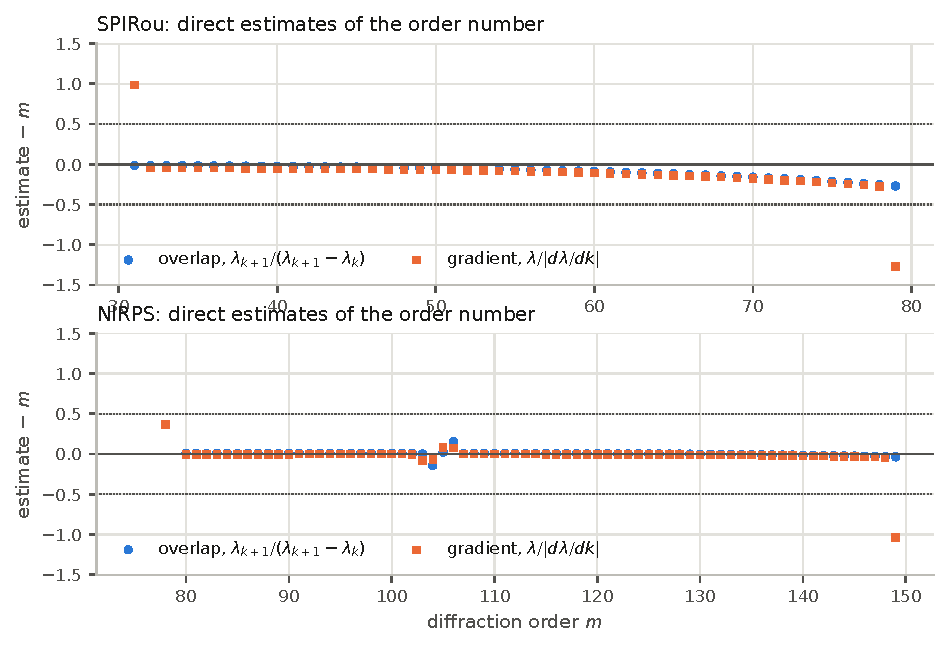
\includegraphics[width=\textwidth]{orders_direct.pdf}
\caption{Direct estimates of the order number from the wavelength solution, minus the adopted integer order. Blue: overlap of consecutive orders (Eq.~\ref{eq:overlap}). Orange: $\lambda/|d\lambda/dk|$, whose first and last points use a one-sided difference. Dotted lines mark $\pm0.5$.}
\label{fig:orderdirect}
\end{figure}

{\small
\begin{longtable}{rrrrrrr}
\caption{Order identification for SPIRou, as computed by \code{mkblaze.py}. $k$: index in the file. $m$: adopted diffraction order. $\lambda^{\rm peak}$: wavelength of the blaze maximum. $m\lambda^{\rm peak}$: its product with $m$. $\lambda^{\rm c}$: wavelength of the central pixel. $m_{\rm ov}$: overlap estimate (Eq.~\ref{eq:overlap}). $m_{\rm grad}$: $\lambda^{\rm c}/|d\lambda^{\rm c}/dk|$.}\label{tab:orders}\\
\toprule
$k$ & $m$ & $\lambda^{\rm peak}$ [nm] & $m\lambda^{\rm peak}$ [nm] & $\lambda^{\rm c}$ [nm] & $m_{\rm ov}$ & $m_{\rm grad}$ \\
\midrule
\endfirsthead
\toprule
$k$ & $m$ & $\lambda^{\rm peak}$ [nm] & $m\lambda^{\rm peak}$ [nm] & $\lambda^{\rm c}$ [nm] & $m_{\rm ov}$ & $m_{\rm grad}$ \\
\midrule
\endhead
\bottomrule
\endfoot
\rows{orders_SPIRou.tex}
\end{longtable}
}

%======================================================================
\section{The model}
\label{sec:model}

The number of photo-electrons recorded in pixel $x$ of order $m$ is modelled as
\begin{equation}
N(m,x) = B_\gamma(\lambda;T)\;\mathcal{T}(\lambda)\;E(m,\lambda)\;\left|\frac{d\lambda}{dx}\right|,
\qquad \lambda = \lambda_m(x).
\label{eq:model}
\end{equation}
Figure~\ref{fig:components} shows the four terms for SPIRou.

\subsection{The lamp, in photons}

The flat lamp is taken to be a blackbody at $T = \spTeff$~K. The detector counts photons, not energy, so the relevant quantity is the Planck function divided by the photon energy $hc/\lambda$:
\begin{equation}
B_\gamma(\lambda;T) \propto \frac{1}{\lambda^4\left[\exp\left(hc/\lambda k_{\rm B} T\right)-1\right]}.
\end{equation}
Using the energy form instead would move the peak of the lamp spectrum by a factor of \PeakRatio\ in wavelength. As Section~\ref{sec:teff} shows, $T$ is not constrained by the data once the transmission is free, so its value is a convention.

\subsection{The width of a pixel}

$|d\lambda/dx|$ converts a photon density per unit wavelength into photons per pixel. It is taken from the wavelength solution by finite differences. The solution is not linear, so this term varies by \spDwaveVar\% along a typical SPIRou order (median over orders). It tilts each order and pulls its maximum to the blue.

\subsection{The grating envelope}
\label{sec:envelope}

The blaze proper is the diffraction pattern of a single groove, $E = \sinc^2\phi$ with $\sinc\phi=\sin\phi/\phi$ \citep{Schroeder2000}. For a grating used close to Littrow, at incidence and diffraction angle $\theta$ from the grating normal with blaze angle $\theta_{\rm b}$, the phase across an illuminated groove width $W$ is
\begin{equation}
\phi = \frac{2\pi W}{\lambda}\,\sin(\theta-\theta_{\rm b}).
\end{equation}
Shadowing by the neighbouring groove limits the illuminated width to $W = d\cos\theta_{\rm b}$. Here $d$ is the groove spacing. Write $C = 2d\sin\theta_{\rm b}$ (any out-of-plane angle $\gamma$ multiplies it by $\cos\gamma$) and $s = m\lambda/C$, which is 1 at the blaze peak. The grating equation then gives $\sin\theta = s\sin\theta_{\rm b}$, and
\begin{equation}
\frac{\phi}{\pi} = \frac{m\cos\theta_{\rm b}}{s}\left[s\cos\theta_{\rm b}-\sqrt{1-s^2\sin^2\theta_{\rm b}}\right].
\label{eq:exact}
\end{equation}
With $e = s-1$, which is 0 at the peak and about $\pm1/m$ at the edges of an order, the expansion to second order is (Appendix~\ref{app:expansion})
\begin{equation}
\frac{\phi}{\pi} = m\left[e + \left(\tfrac12\tan^2\theta_{\rm b}-1\right)e^2\right] + O(m e^3).
\label{eq:expansion}
\end{equation}
The model uses the second-order form, with two shape parameters:
\begin{equation}
E(m,\lambda) = \sinc^2\!\left[\pi\beta m\left(e+\alpha e^2\right)\right],\qquad e = \frac{m\lambda}{C(\lambda)}-1.
\label{eq:envelope}
\end{equation}
$\beta$ scales the illuminated width: its first zeros fall at $e = \pm1/(\beta m)$, that is $\pm1/\beta$ free spectral ranges from the peak. $\beta=1$ is the fully illuminated groove. The asymmetry $\alpha$ is $\tfrac12\tan^2\theta_{\rm b}-1$ for a Littrow grating: $+1$ for an R2 grating ($\tan\theta_{\rm b}=2$, SPIRou) and $+7$ for an R4 ($\tan\theta_{\rm b}=4$, NIRPS, whose grating has a nominal blaze angle of $76^\circ$; \citealt{LFW2017}). It is nevertheless left free, because the data do not follow that relation (Section~\ref{sec:littrow}).

Over the extent of an order ($m=55$, $|\phi/\pi|$ up to 0.8), Eq.~\ref{eq:expansion} reproduces Eq.~\ref{eq:exact} to $\ExpAccA$ in $\phi/\pi$ for $\theta_{\rm b}=30^\circ$ and $\ExpAccB$ for $63.4^\circ$, but only to $\ExpAccC$ for $76^\circ$. For an R4 grating the third-order term is not negligible. With $\alpha$ free, the fit absorbs it into an effective asymmetry.

\subsection{A chromatic grating constant}
\label{sec:chromatic}

The grooves are the same for every order, but the angle at which the beam meets them need not be. SPIRou's cross-disperser is a train of two ZnSe prisms and one Infrasil prism, used in double pass: the collimated beam crosses it before the \'echelle and again after \citep{Donati2020,Thibault2012}. The beam therefore reaches the grating already dispersed. Its out-of-plane angle $\gamma$ depends on wavelength, and so does $C = 2d\sin\theta_{\rm b}\cos\gamma$. To first order,
\begin{equation}
C(\lambda) = c_0 + c_1\,(\lambda-\lambda_{\rm ref}) = a_0 + a_1\lambda,
\label{eq:chromatic}
\end{equation}
The model uses this form. Here $\lambda_{\rm ref}$ is the median wavelength of the fitted pixels (\spLref~nm for SPIRou, \niLref~nm for NIRPS). Writing $C$ around $\lambda_{\rm ref}$ decorrelates the two coefficients during the fit; $a_0 = c_0 - c_1\lambda_{\rm ref}$ and $a_1 = c_1$ are derived from them. In an exploratory test, run outside the scripts of this report, a quadratic term lowered the SPIRou fit cost by a further 30\%. It is not included.

\subsection{The transmission}
\label{sec:transmission}

$\mathcal{T}(\lambda)$ gathers everything else: filters, coatings, fibre, detector quantum efficiency and the absolute scale. It is by far the largest term, varying by a factor of \spTransRange\ across SPIRou. It is modelled as a spline in $\ln\mathcal{T}$ with one knot per order, placed at the observed maximum of the order. The value of knot $k$ is
\begin{equation}
\ln\mathcal{T}_k = \operatorname*{median}_{|x-x_k^{\rm peak}|\le 50}\left[\ln N_{\rm obs}(x) - \ln\left(B_\gamma\,E\,|d\lambda/dx|\right)\right],
\end{equation}
and its wavelength is the median wavelength over the same pixels. The other three terms must be divided out first. The flux at the peak contains them too, and would otherwise count them twice. By default the spline is linear between knots, and its end segments continue beyond the first and last knot. A polynomial in $\ln\mathcal{T}$ is available as an alternative (Section~\ref{sec:comparison}).

\begin{figure}[p]
\centering
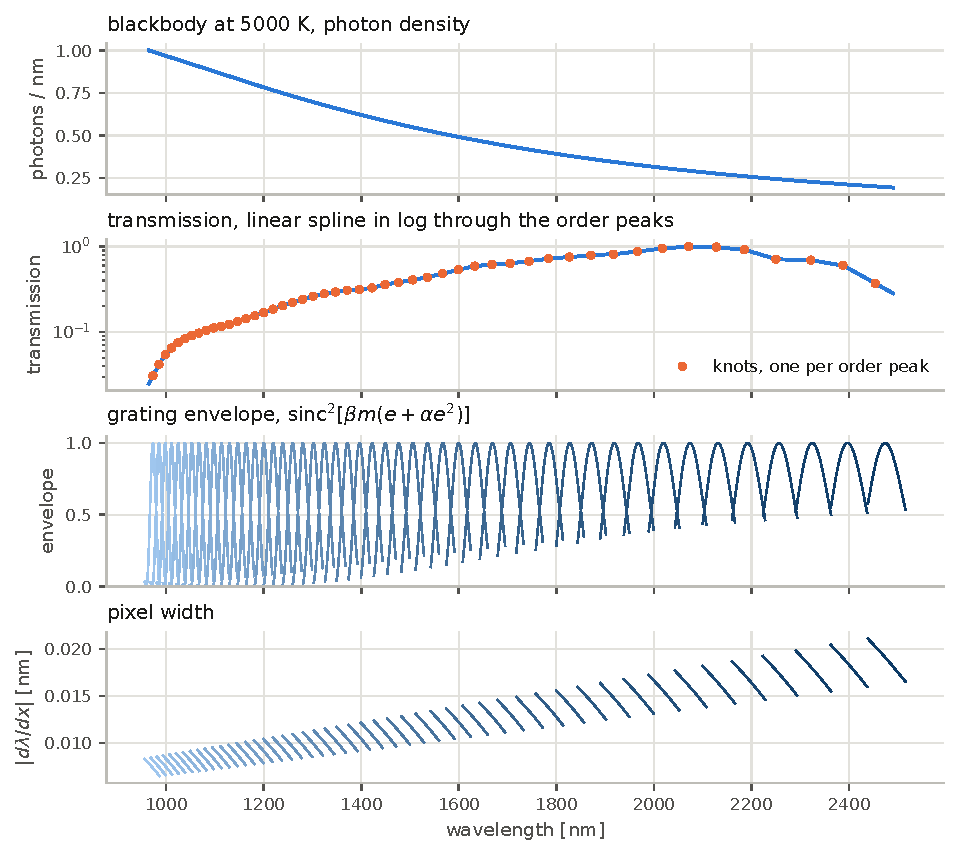
\includegraphics[width=\textwidth]{components_SPIRou.pdf}
\caption{The four terms of the SPIRou model, at the maximum a posteriori. From top to bottom: the photon blackbody, the transmission with its knots, the grating envelopes, and the pixel width. Colour runs from the bluest order to the reddest.}
\label{fig:components}
\end{figure}

%======================================================================
\section{Fitting}
\label{sec:fit}

\subsection{Method}

\code{fit\_blaze.py} has four non-linear parameters, $(c_0, c_1, \beta, \alpha)$. The transmission never enters the non-linear solver. For a given set of grating parameters, the spline knots are read directly off the data, or a polynomial is solved by linear least squares, since $\ln\mathcal{T}$ enters linearly (variable projection). The residual is $\ln N_{\rm obs}-\ln N$. It is minimised with \code{scipy.optimize.least\_squares} \citep{Virtanen2020} using a soft-L1 loss with a scale of 0.05. Three passes follow, each rejecting pixels beyond 5 times the residual rms. $C$ starts flat, at the mean of $m\lambda^{\rm peak}$, and the envelope starts symmetric ($\alpha=0$, $\beta=1$). All pixels are fitted, since the red limit of the fitted range is set at 2500~nm, beyond the data. The model is then evaluated on every pixel, including the \spValidPct\% of SPIRou pixels that have a blaze and the rest that do not.

\subsection{Results}

For SPIRou, the fit gives $C(\lambda) = \spBestAzero\;\spBestAone\,\lambda$~nm, a change of $\spBestChange\%$ across the array. It also gives $\beta = \spBestBeta$ and $\alpha = \spBestAsym$. The residual $N_{\rm obs}/N-1$ has a median absolute value of \spFitMed\% and an rms of \spFitRms\%. The rms is dominated by a few orders at the ends of the array: the median of the per-order rms is \spFitPerOrder\%, and the worst orders are \spFitWorst. At the maximum a posteriori of Section~\ref{sec:mcmc}, which weights the residuals differently, the median residual is \spMedRel\%, the median per-order rms \spMedPerOrder\%, and half of the orders have an rms between \spPerOrderQlo\ and \spPerOrderQhi\%. Figures~\ref{fig:fit} and \ref{fig:zoom} show that model.

For NIRPS: $C(\lambda) = \niBestAzero\;\niBestAone\,\lambda$~nm ($\niBestChange\%$), $\beta = \niBestBeta$, $\alpha = \niBestAsym$, with a median residual of \niFitMed\%, an rms of \niFitRms\% and a median per-order rms of \niFitPerOrder\%. The worst orders are \niFitWorst. They lie at the red end of H and on either side of the J/H gap, where the transmission changes within a single free spectral range and one knot per order cannot follow it.

\begin{figure}[t]
\centering
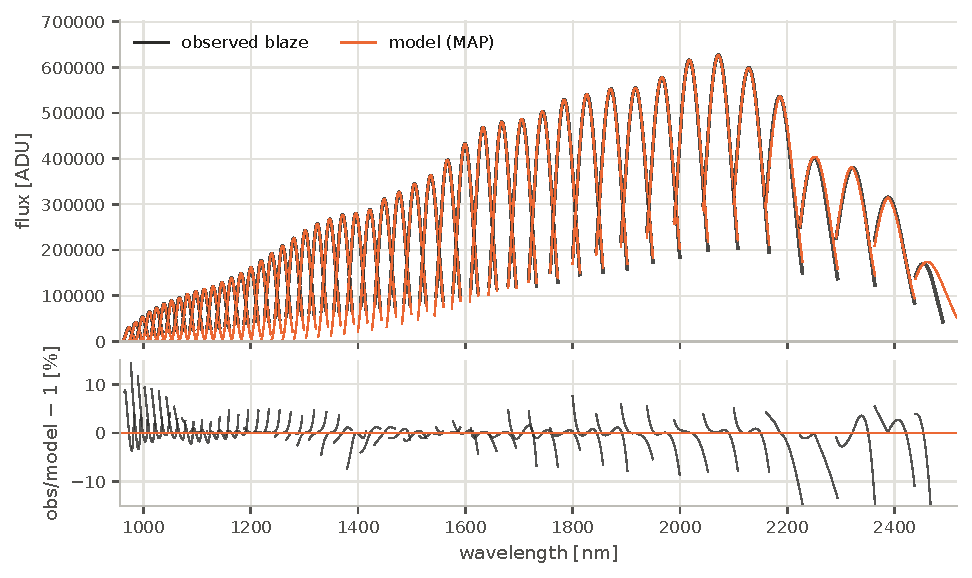
\includegraphics[width=\textwidth]{fit_SPIRou.pdf}
\caption{SPIRou: the observed blaze (black) and the model at the maximum a posteriori (orange), with the relative residual below.}
\label{fig:fit}
\end{figure}

\begin{figure}[t]
\centering
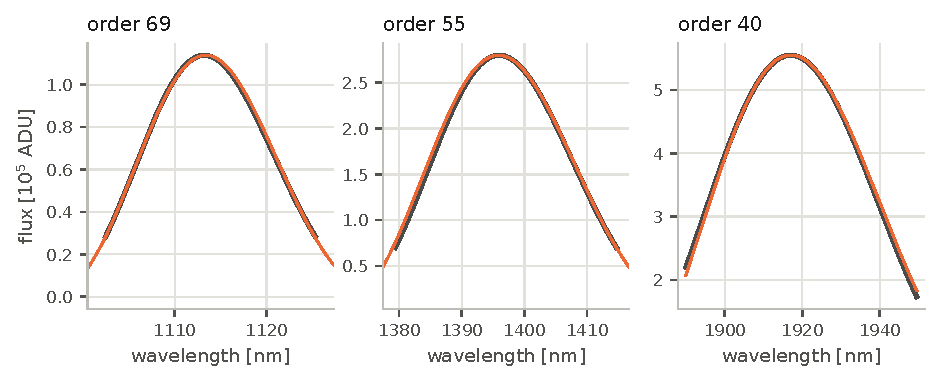
\includegraphics[width=\textwidth]{zoom_SPIRou.pdf}
\caption{Three SPIRou orders at full scale. The model is drawn over the whole order, including the pixels where the pipeline blaze is undefined.}
\label{fig:zoom}
\end{figure}

\subsection{The chromatic term and the peak positions}
\label{sec:peaks}

With $C$ held constant, the observed maxima of the SPIRou orders sit systematically bluer than the model, by $\spPkConstMean\pm\spPkConstRms$ pixels over orders 36 to 79. The offset grows towards the red and reaches \spPkConstMax\ pixels at order \spPkConstMaxOrder. With the chromatic $C$ the offset becomes $\spPkMapMean\pm\spPkMapRms$ pixels (Figure~\ref{fig:peaks}). What remains is a smooth pattern, from $\spPkMapFirst$ pixels at order \spMfirst\ to $+\spPkMapMaxPos$ at order \spPkMapMaxPosOrder, which a quadratic term in $C(\lambda)$ would absorb.

The product $m\lambda^{\rm peak}$ drifts by \spPeakDrift~nm across SPIRou, far more than the change of $C$ itself (\spCblue\ to \spCred~nm, i.e. \spCdrop~nm). The rest of the drift comes from the slope of the lamp spectrum and of $|d\lambda/dx|$, which pulls each observed maximum off the true blaze peak. The model reproduces this drift, because it contains both effects.

If the published SPIRou grating is taken at face value (\spGrooves\ grooves/mm, R2, so $2d\sin\theta_{\rm b} = \spTwoDsin$~nm), the fitted $C(\lambda)$ corresponds to an out-of-plane angle growing from $\gamma = \spGammaBlue^\circ$ at the blue end to $\spGammaRed^\circ$ at the red end. That is a change of $\spGammaDelta^\circ$. This estimate is illustrative, as it assumes an exact Littrow geometry in the dispersion plane. It is nonetheless consistent with the angular spread a prism cross-disperser imposes before the grating.

\begin{figure}[t]
\centering
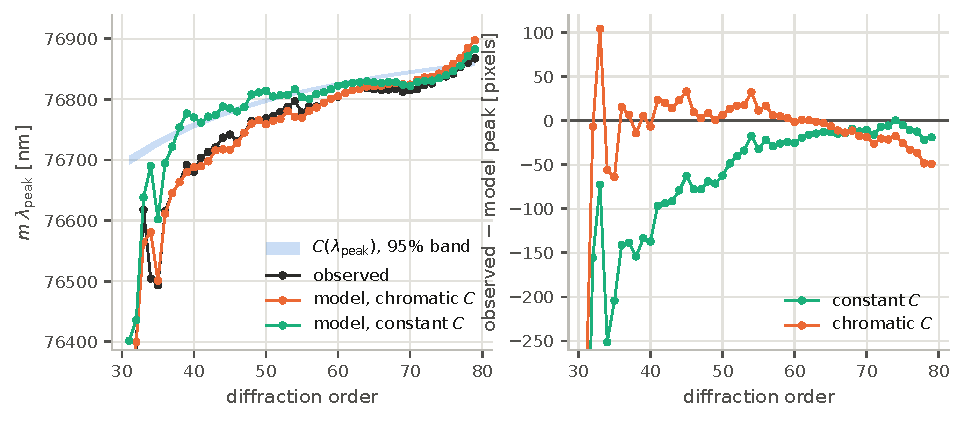
\includegraphics[width=\textwidth]{peaks_SPIRou.pdf}
\caption{SPIRou. Left: $m\lambda$ at the maximum of each order, observed (black), for the model with a chromatic $C$ (orange), and for the model with a constant $C$ (green). The blue band is the 95\% posterior of $C(\lambda)$ at the peak wavelength. Right: offset between the observed and modelled maxima, in pixels.}
\label{fig:peaks}
\end{figure}

\subsection{Model comparison}
\label{sec:comparison}

Table~\ref{tab:comparison} lists the results of \code{fit\_blaze.py} re-run with one setting changed at a time. Three conclusions follow.
\begin{itemize}
\item \textbf{The chromatic term matters regardless of the transmission model.} With either the spline or the polynomial, it lowers the median residual and the per-order rms. The change of $C$ it returns barely depends on the transmission model: $\spChangeRangeHi$ to $\spChangeRangeLo\%$ for SPIRou and $\niChangeRangeHi$ to $\niChangeRangeLo\%$ for NIRPS.
\item \textbf{The spline wins on the typical pixel.} The order~21 polynomial keeps a lower global rms on SPIRou, because it spreads its error into the wings, where the spline answers only to the peak.
\item \textbf{The decisive difference is outside the fitted range.} With the red limit moved to 2400~nm on SPIRou, the linear spline misses the unseen pixels by a median of \spExtLin\%, the cubic spline by \spExtCub\%, and the order~21 polynomial by $\spExtPoly\%$. The linear and cubic splines differ by \spCubDiffMed\% in median residual inside the fitted range. The linear one is the default because it cannot overshoot.
\end{itemize}

\begin{table}[t]
\centering
\caption{\code{fit\_blaze.py} with one setting changed at a time. Residuals are $N_{\rm obs}/N-1$ in \%, over the fitted pixels. $\Delta C$ is the change of $C$ across the array, in \%.}
\label{tab:comparison}
\small
\begin{tabular}{lrrrrrr}
\toprule
model & median & rms & per-order & $\Delta C$ [\%] & $\alpha$ & $\beta$ \\
\midrule
\multicolumn{7}{l}{\emph{SPIRou}}\\
\rows{comparison_SPIRou.tex}
\midrule
\multicolumn{7}{l}{\emph{NIRPS}}\\
\rows{comparison_NIRPS.tex}
\bottomrule
\end{tabular}
\end{table}

%======================================================================
\section{MCMC characterisation}
\label{sec:mcmc}

\subsection{What the residuals look like}

A likelihood needs a noise model, and the blaze has almost no noise: \apero\ delivers a smoothed product. The residuals are model errors, and two of their properties shape the likelihood (Figure~\ref{fig:resid}).
\begin{itemize}
\item \textbf{They are correlated along the orders.} The autocorrelation of $\ln(N_{\rm obs}/N)$, with each order's mean removed, falls to $1/e$ at $\ell = \spCorr$~pixels for SPIRou and $\niCorr$ for NIRPS. A SPIRou order of about 3300 fitted pixels therefore holds only about five independent residuals, and the whole array about \spNeff.
\item \textbf{They are heavy-tailed and skewed.} For SPIRou, the excess kurtosis is \spKurt\ and the skewness $\spSkew$. The rms is \spResStd\%, against a robust width (1.4826 times the median absolute deviation) of \spMad\%. A Student-$t$ distribution fits the residuals with $\nu = \spNu$ degrees of freedom and a scale of \spTscale\%. For NIRPS, $\nu = \niNu$, close to a Lorentzian, because a few orders are missed by factors of several.
\end{itemize}

\begin{figure}[t]
\centering
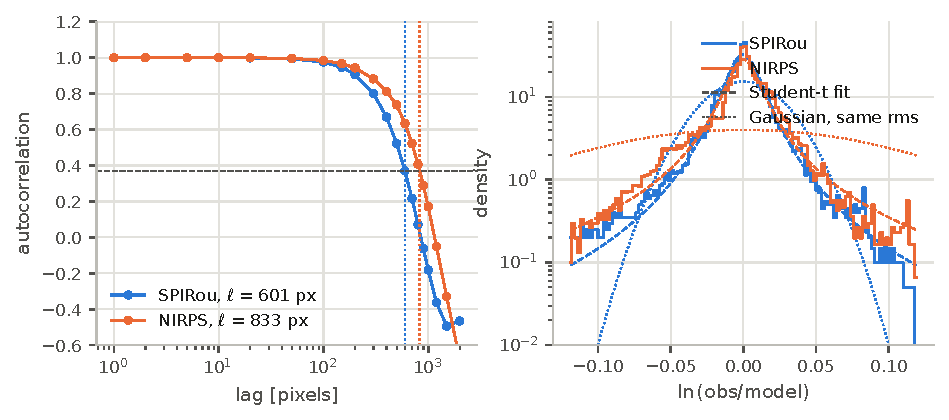
\includegraphics[width=\textwidth]{residual_stats.pdf}
\caption{Left: autocorrelation of the log residual along the orders. The dotted verticals mark the $1/e$ length. Right: distribution of the log residual, with the Student-$t$ fit (dashed) and a Gaussian of the same rms (dotted).}
\label{fig:resid}
\end{figure}

\subsection{Likelihood}

The likelihood is a Student-$t$ distribution on the log residuals $r_i$, with $\nu$ fixed at the value above and a free scale $s$. It is evaluated on the fitted pixels decimated by $d=\spDec$ along each order: \spNlike\ pixels for SPIRou. It is also tempered by $d/\ell$, so that the sum counts independent samples rather than correlated pixels:
\begin{equation}
\ln\mathcal{L} = \frac{d}{\ell}\sum_i\left[\ln\frac{\Gamma\left(\frac{\nu+1}{2}\right)}{\Gamma\left(\frac{\nu}{2}\right)\sqrt{\nu\pi}} - \ln s - \frac{\nu+1}{2}\ln\left(1+\frac{r_i^2}{\nu s^2}\right)\right].
\label{eq:like}
\end{equation}
For SPIRou the tempering factor is \spTemper. The transmission is profiled: at every call, the knots are recomputed from the full-resolution peak windows (\spNwin\ pixels for SPIRou) for the current grating parameters. The pixel set is the one kept by the 5$\sigma$ clipping at the best fit. The likelihood reproduces the stored model to $\spLikeCheck$ and its knots to $\spKnotCheck$ in $\ln\mathcal{T}$, and it takes \spLikeMs~ms per call.

The priors are uniform: $c_0$ within 10\% of the best fit, $|c_1| < c_0/\lambda_{\rm ref}$, $0.1<\beta<5$, $|\alpha|<100$ and $-12<\ln s<2$. None of them is close to the posterior.

Posterior widths scale as $\sqrt{\ell/d}$ with the tempering. The choice of $\ell$ is the main assumption of the analysis, which is why Section~\ref{sec:jack} checks the widths with a jackknife that does not depend on it.

\subsection{Sampling}

The posterior is sampled with \code{emcee} \citep{ForemanMackey2013}, the affine-invariant ensemble sampler of \citet{Goodman2010}, with \spNwalkers\ walkers started in a small ball around the maximum a posteriori. The chain grows in blocks of 2000 steps. It stops when it is longer than 50 autocorrelation times and the autocorrelation time has changed by less than 2\% since the previous block. For SPIRou this took \spNsteps\ steps (\spStepsOverTau\ autocorrelation times), with integrated autocorrelation times between \spTauMin\ and \spTauMax\ steps and an acceptance fraction of \spAcc. The first \spBurn\ steps (three autocorrelation times) are discarded and the chain is thinned by \spThin, which leaves \spNsamples\ samples. For NIRPS: \niNsteps\ steps, $\tau \le \niTauMax$, acceptance \niAcc, \niNsamples\ samples. The chains are shown in Appendix~\ref{app:chains}.

\subsection{Posteriors}

Table~\ref{tab:posterior} gives the posterior medians and 68\% intervals. Figures~\ref{fig:cornersp} and \ref{fig:cornerni} show the corner plots \citep{ForemanMackey2016}. The strongest correlation in the SPIRou posterior is between \spCorrPair\ ($\rho=\spCorrPairVal$), and in the NIRPS posterior between \niCorrPair\ ($\rho=\niCorrPairVal$). $c_0$ and $c_1$ are nearly independent ($\rho=\spCorrCzeroCone$ and $\niCorrCzeroCone$), as intended by the choice of $\lambda_{\rm ref}$.

The chromatic change of $C$ is detected at $\spChangeSig\sigma$ in SPIRou and $\niChangeSig\sigma$ in NIRPS with the posterior widths, and still at $\spChangeSigJack\sigma$ and $\niChangeSigJack\sigma$ with the jackknife ones. Figure~\ref{fig:clambda} shows $C(\lambda)$ relative to its value at $\lambda_{\rm ref}$ for both instruments.

\begin{table}[t]
\centering
\caption{Posterior medians and 68\% intervals, and jackknife uncertainties over orders. $c_0 = C(\lambda_{\rm ref})$ and $c_1 = a_1 = dC/d\lambda$. $d\ln C/d\ln\lambda$ is evaluated at $\lambda_{\rm ref}$ and given in units of $10^{-3}$. $\Delta C$ is the change across the array. $c_0$ and $a_0$ are in nm and $c_1$ in nm per nm. $\beta$, $\alpha$ and $\ln s$ are dimensionless, $s$ being the Student-$t$ scale of the log residual.}
\label{tab:posterior}
\small
\begin{tabular}{lcccc}
\toprule
 & \multicolumn{2}{c}{SPIRou} & \multicolumn{2}{c}{NIRPS} \\
 & posterior & jackknife $\sigma$ & posterior & jackknife $\sigma$ \\
\midrule
$c_0 = C(\lambda_{\rm ref})$ [nm] & $\spCzero$ & $\spJackCzero$ & $\niCzero$ & $\niJackCzero$ \\
$c_1 = a_1$ & $\spCone$ & $\spJackCone$ & $\niCone$ & $\niJackCone$ \\
$\beta$ & $\spBeta$ & $\spJackBeta$ & $\niBeta$ & $\niJackBeta$ \\
$\alpha$ & $\spAsym$ & $\spJackAsym$ & $\niAsym$ & $\niJackAsym$ \\
$\ln s$ & $\spLns$ & & $\niLns$ & \\
\midrule
$a_0$ [nm] & $\spAzero$ & $\spJackAzero$ & $\niAzero$ & $\niJackAzero$ \\
$d\ln C/d\ln\lambda$ [$10^{-3}$] & $\spDlnc$ & $\spJackDlnc$ & $\niDlnc$ & $\niJackDlnc$ \\
$\Delta C$ [\%] & $\spChange$ & $\spJackChange$ & $\niChange$ & $\niJackChange$ \\
\bottomrule
\end{tabular}
\end{table}

\begin{figure}[p]
\centering
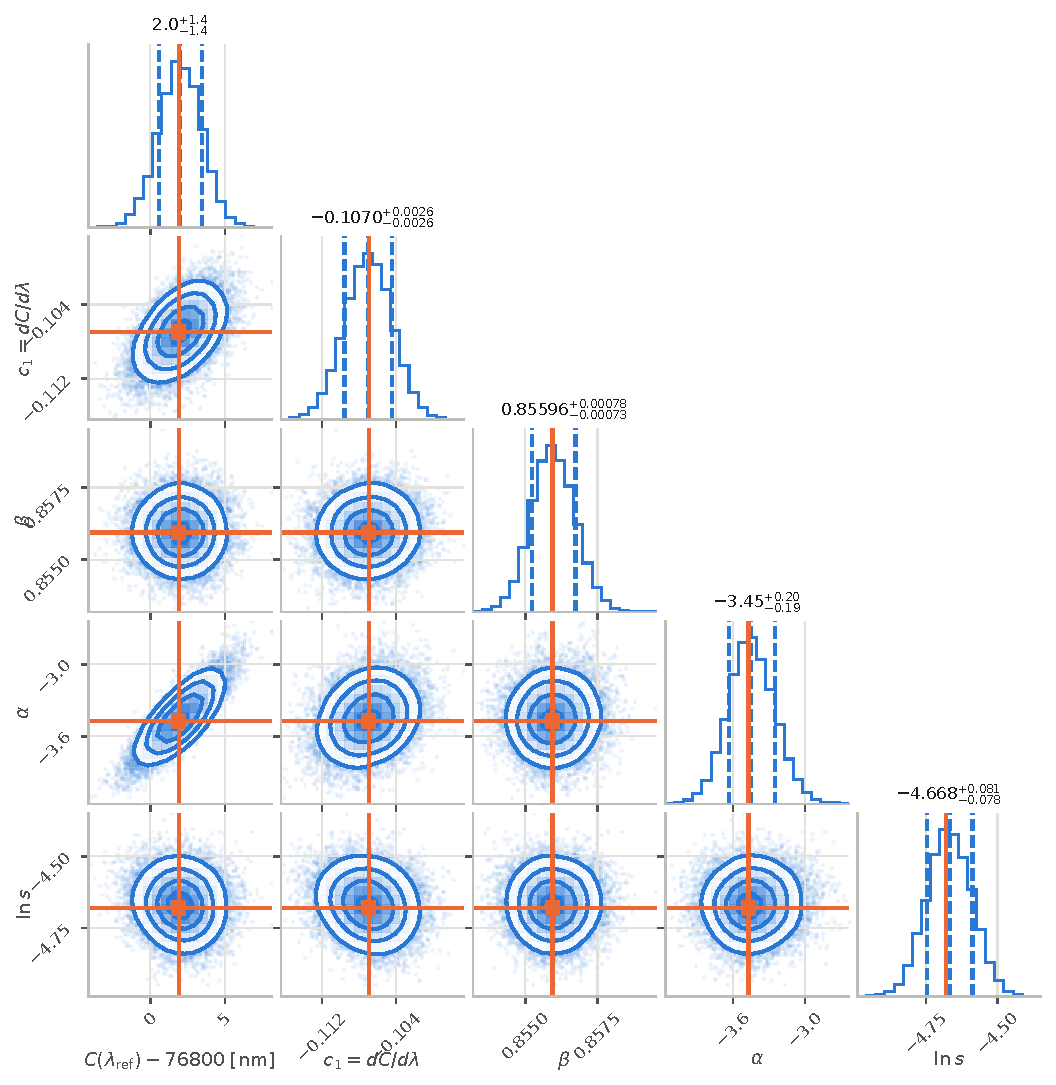
\includegraphics[width=0.92\textwidth]{corner_SPIRou.pdf}
\caption{SPIRou posterior. Orange lines mark the maximum a posteriori.}
\label{fig:cornersp}
\end{figure}

\begin{figure}[p]
\centering
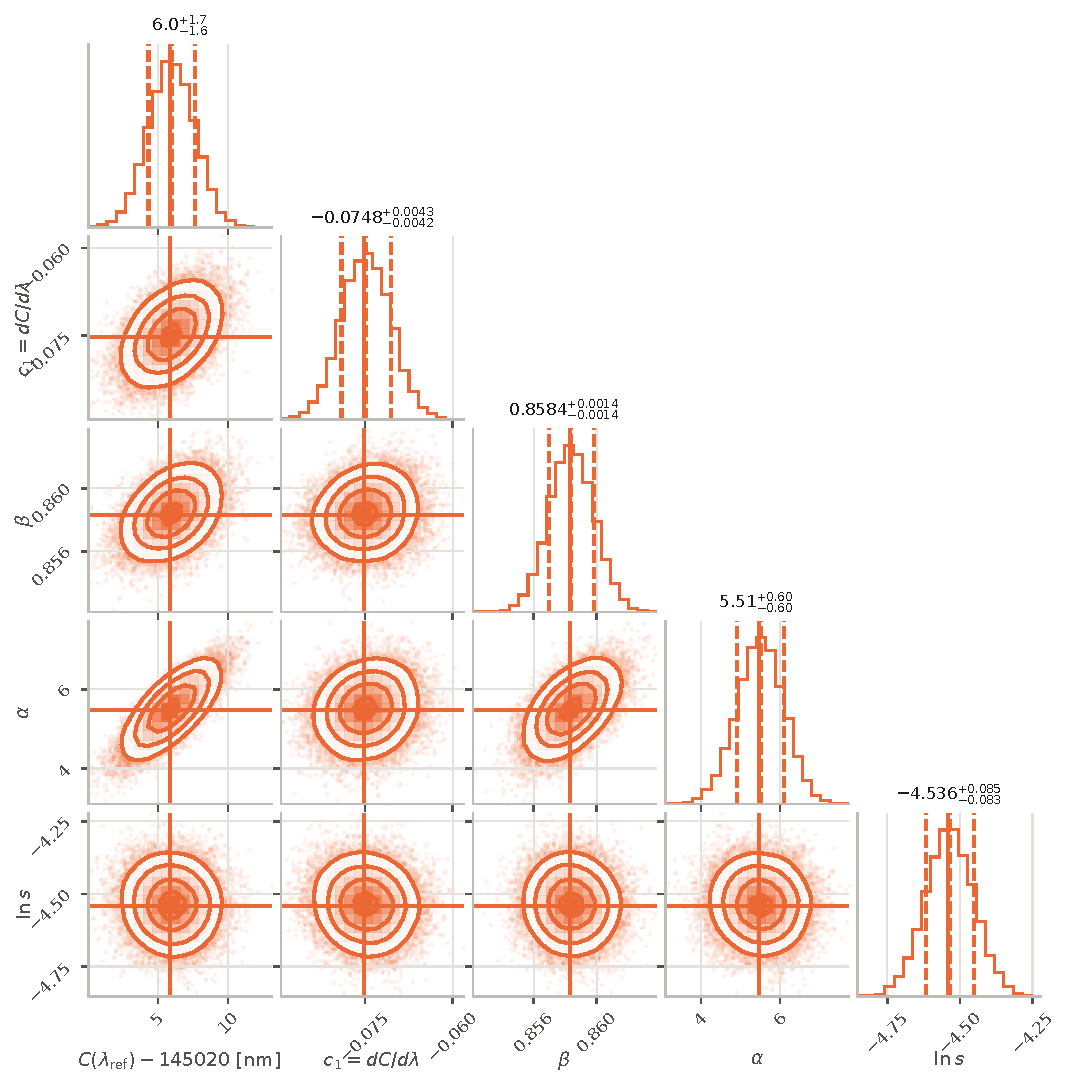
\includegraphics[width=0.92\textwidth]{corner_NIRPS.pdf}
\caption{NIRPS posterior. Orange lines mark the maximum a posteriori.}
\label{fig:cornerni}
\end{figure}

\begin{figure}[t]
\centering
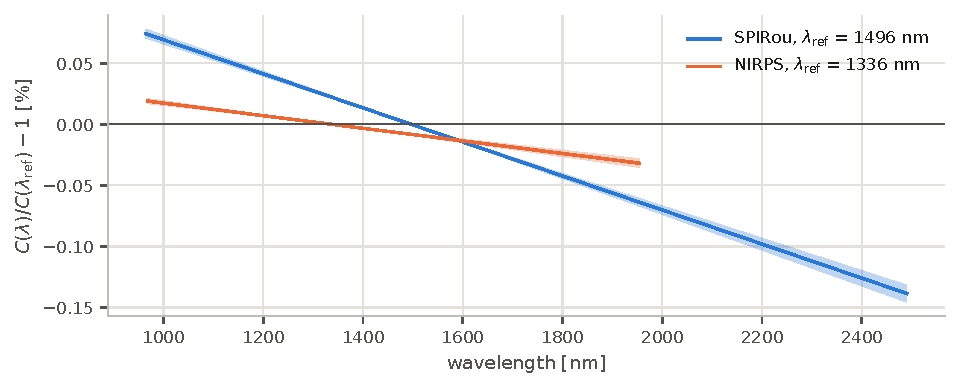
\includegraphics[width=\textwidth]{c_lambda.pdf}
\caption{The grating constant relative to its value at the reference wavelength. The line is the posterior median and the band the 95\% interval.}
\label{fig:clambda}
\end{figure}

\subsection{Jackknife over orders}
\label{sec:jack}

Leaving out one order at a time and maximising the posterior again gives an estimate of the uncertainty. It does not depend on $\ell$, since the tempering scales the likelihood without moving its maximum. It captures how much the answer depends on the particular orders at hand, which is the dominant source of error for a model limited by systematics. The jackknife uncertainty is
\begin{equation}
\sigma^2_{\rm JK} = \frac{n-1}{n}\sum_{j=1}^{n}\left(\theta_{(j)}-\bar\theta\right)^2 .
\end{equation}
Table~\ref{tab:posterior} compares it with the posterior width. For SPIRou the ratio of jackknife to posterior uncertainty is \spRatioCzero\ for $c_0$, \spRatioCone\ for $c_1$, \spRatioBeta\ for $\beta$ and \spRatioAsym\ for $\alpha$. For NIRPS it is \niRatioCzero, \niRatioCone, \niRatioBeta\ and \niRatioAsym. The jackknife is systematically the larger, by a factor between \MinRatio\ and \MaxRatio. The residuals contain structure that the tempered likelihood only partly accounts for, and the jackknife uncertainties are the safer figures to quote. Figure~\ref{fig:jacksp} shows how far each parameter moves when each order is left out. Since $\sigma_{\rm JK}\simeq\sqrt{n-1}$ times the rms of these shifts, the individual shifts are small compared with the uncertainty; what matters is that no single order stands out.

\begin{figure}[t]
\centering
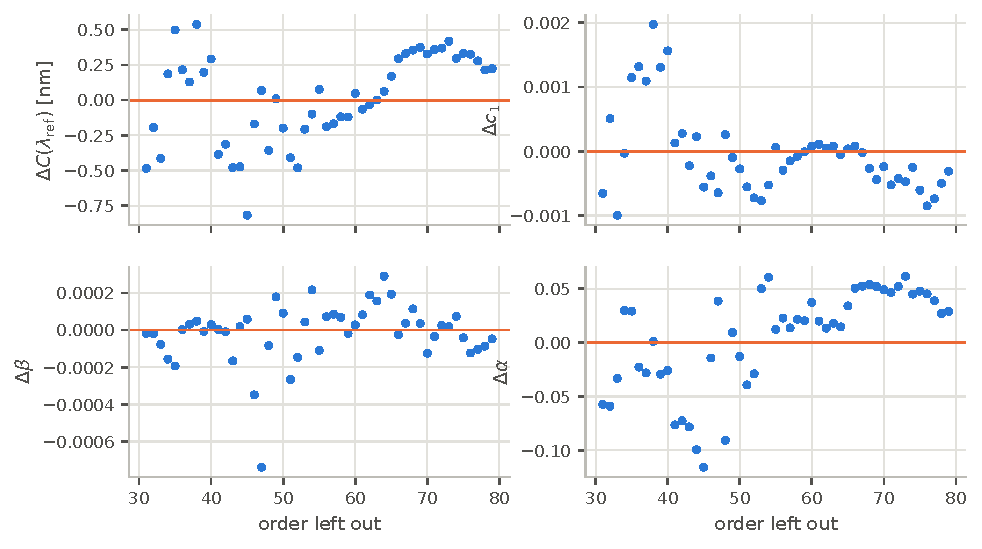
\includegraphics[width=\textwidth]{jackknife_SPIRou.pdf}
\caption{SPIRou jackknife: shift of the maximum a posteriori when each order is left out in turn.}
\label{fig:jacksp}
\end{figure}

\subsection{Profile tests}
\label{sec:profiles}

Profiles compare the maximum of the tempered likelihood with and without a constraint. As a rough guide, $2\Delta\ln\mathcal{L}$ can be read as a $\chi^2$ with one degree of freedom.

\paragraph{No chromatic term.} Forcing $c_1=0$ costs $\Delta\ln\mathcal{L} = \spDlpConst$ for SPIRou and \niDlpConst\ for NIRPS. Even after the tempering, a constant $C$ is excluded.

\paragraph{Littrow asymmetry.}
\label{sec:littrow}
The Littrow value of $\alpha$ for the nominal grating is $\spAsymLittrow$ for SPIRou's R2 and $\niAsymLittrow$ for NIRPS's R4. The two instruments behave differently.
\begin{itemize}
\item \textbf{SPIRou.} Imposing the Littrow value costs $\Delta\ln\mathcal{L} = \spDlpLittrow$. The posterior, $\alpha = \spAsym$, lies below $-1$, which no real blaze angle can produce in Eq.~\ref{eq:expansion}. With $C$ held constant, the fit had landed close to the Littrow value, at $\alpha\approx+0.9$ (Table~\ref{tab:comparison}). That was the asymmetry standing in for the missing chromatic term.
\item \textbf{NIRPS.} The Littrow value is only mildly disfavoured, with $\Delta\ln\mathcal{L} = \niDlpLittrowDec$. The posterior, $\alpha = \niAsym$, lies $\niLittrowSig\sigma$ below it with the posterior width and $\niLittrowSigJack\sigma$ with the jackknife one. Two caveats weaken the comparison. For an R4 grating, the second-order envelope is itself only accurate to $\ExpAccC$ (Section~\ref{sec:envelope}). And $\alpha$ depends on how the residuals are weighted: it is $\niBestAsym$ with the soft-L1 loss of \code{fit\_blaze.py} and $\niAsym$ with the Student-$t$ likelihood.
\end{itemize}
$\alpha$ is therefore best read as a shape parameter, and it measures the blaze angle at most for NIRPS. Plausible contributors are departures from Littrow in the dispersion plane, the groove profile, the illumination of the pupil and the extraction; the data do not separate them.

\paragraph{Lamp temperature.}
\label{sec:teff}
Between 3000 and 8000~K, the maximum likelihood changes by at most \spTeffDlpMid\ for SPIRou and \niTeffDlpMid\ for NIRPS, and by at most \spTeffDlpMax\ over the whole 2500 to 30\,000~K grid for SPIRou. The spline absorbs the slope of the blackbody, and only its curvature within one free spectral range is left to constrain $T$. The grating parameters barely move: across the grid, none of them shifts by more than $\spTeffShift$ of its posterior width for SPIRou, or $\niTeffShift$ for NIRPS (Figure~\ref{fig:teff}). The lamp temperature is not measurable from a blaze with a free transmission, and fixing it costs nothing.

\begin{figure}[t]
\centering
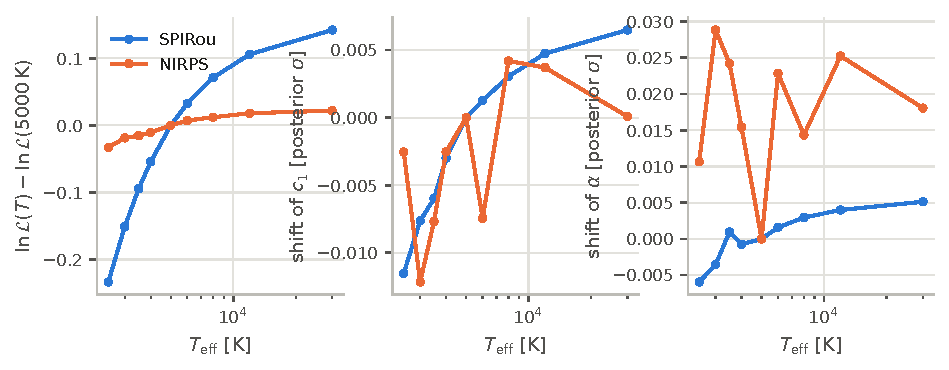
\includegraphics[width=\textwidth]{teff_profile.pdf}
\caption{Profile in lamp temperature. Left: log-likelihood relative to the adopted 5000~K. Centre and right: shift of the chromatic slope and of the asymmetry, in units of their posterior widths.}
\label{fig:teff}
\end{figure}

%======================================================================
\section{NIRPS}
\label{sec:nirps}

The same code, unchanged, identifies the NIRPS orders as \niMfirst\ to \niMlast\ and fits $C(\lambda)$, $\beta = \niBeta$ and $\alpha = \niAsym$. The chromatic change, $\niChange\%$, is \ChangeRatio\ times smaller than on SPIRou. The fit is shown in Figure~\ref{fig:fitni}. The median residual of \niMedRel\% is lower than for SPIRou, while the global rms of \niRmsRel\% is much higher. It is dominated by the orders beyond 1850~nm and around the J/H gap, where the observed blaze deviates from the model by up to several hundred per cent at the order edges. This contrast is also why the NIRPS residuals are nearly Lorentzian.

\begin{figure}[t]
\centering
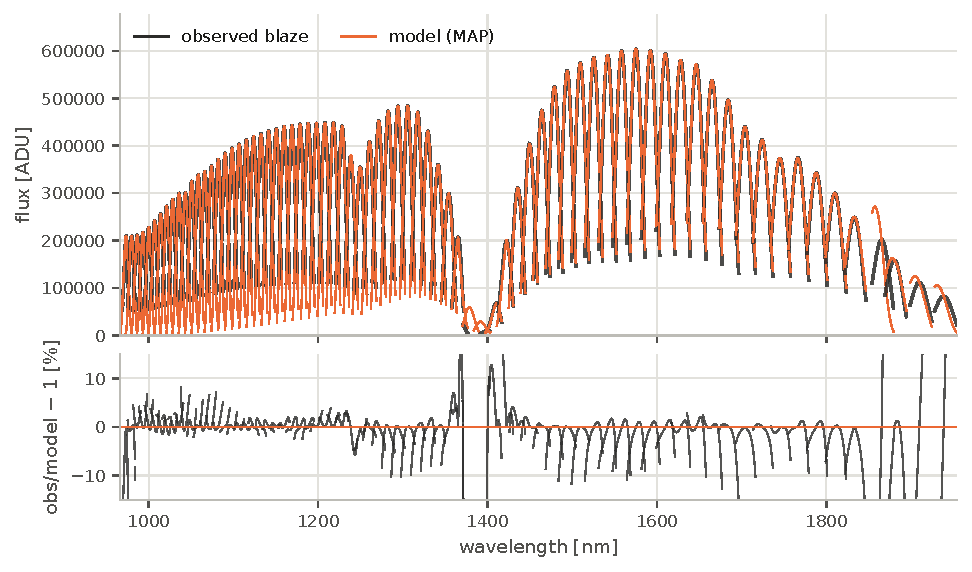
\includegraphics[width=\textwidth]{fit_NIRPS.pdf}
\caption{NIRPS: observed blaze and model, with the relative residual below.}
\label{fig:fitni}
\end{figure}

%======================================================================
\section{Discussion and limitations}
\label{sec:discussion}

\begin{itemize}
\item \textbf{The model works at the percent level with very few parameters.} Four grating parameters and one knot per order describe the SPIRou blaze to a median of \spMedRel\% per pixel, including the positions of the order maxima.
\item \textbf{The chromatic grating constant is real and significant.} It is found with either transmission model, is excluded by neither jackknife nor profile, and has a natural optical origin in SPIRou's double-pass cross-disperser. A linear form leaves a smooth residual in the peak positions that a quadratic term would absorb.
\item \textbf{The asymmetry is a shape parameter.} Earlier versions of the model, with a constant $C$, recovered the nominal R2 and R4 angles. Once $C$ is chromatic, that agreement disappears for SPIRou and holds only at the $\niLittrowSig\sigma$ level for NIRPS, where the asymmetry also depends on how the residuals are weighted.
\item \textbf{The global rms is set by a handful of orders.} These are orders where the transmission changes within one free spectral range, at filter edges and band gaps, which one knot per order cannot follow. The median of the per-order rms is the more representative summary.
\item \textbf{Only the top of each order constrains the envelope.} The \apero\ blaze is cut at 25\% of the maximum, so the wings of the sinc$^2$ are an extrapolation.
\item \textbf{The uncertainties depend on how correlated residuals are counted.} The jackknife gives uncertainties \MinRatio\ to \MaxRatio\ times larger than the MCMC, and those are the ones to quote.
\item \textbf{The lamp temperature is a convention, not a measurement.}
\item \textbf{Outside the fitted range, the model is an extrapolation.} The spline is left free, not clamped, so that the model stays smooth. A high-order polynomial would diverge there.
\end{itemize}

%======================================================================
\section{Conclusions}

A physical model of the \'echelle blaze fits the SPIRou and NIRPS flat fields with four grating parameters and a spline transmission. The diffraction orders are recovered from the wavelength solution alone. The grating constant is chromatic at high significance, with $C$ decreasing by \spChangeAbs\% across SPIRou, and taking this into account brings the model peaks onto the observed ones. The MCMC posterior accounts for the strong correlation of the residuals, and a jackknife over orders gives uncertainties \MinRatio\ to \MaxRatio\ times larger, which are the safer figures. The model is defined on every pixel, so it can extend or replace a thresholded pipeline blaze. The code, the data for SPIRou and the scripts that produce every number and figure of this report are public at \url{https://github.com/eartigau/blaze}.

\paragraph{Software.} numpy \citep{Harris2020}, scipy \citep{Virtanen2020}, astropy \citep{Astropy2022}, emcee \citep{ForemanMackey2013}, corner \citep{ForemanMackey2016}, matplotlib.

\bibliographystyle{plainnat}
\bibliography{blaze_report}

\clearpage
\appendix

%======================================================================
\section{The second-order envelope}
\label{app:expansion}

With $s = 1+e$ and $t=\tan^2\theta_{\rm b}$,
\begin{align}
\sqrt{1-s^2\sin^2\theta_{\rm b}}
&= \cos\theta_{\rm b}\sqrt{1-(2e+e^2)\,t}
= \cos\theta_{\rm b}\left[1 - e\,t - \tfrac12 e^2 t - \tfrac12 e^2 t^2 + O(e^3)\right],\\
s\cos\theta_{\rm b}-\sqrt{1-s^2\sin^2\theta_{\rm b}}
&= \cos\theta_{\rm b}\left[e(1+t) + \tfrac12 e^2 t(1+t) + O(e^3)\right].
\end{align}
Since $\cos^2\theta_{\rm b}(1+t) = 1$ and $1/s = 1-e+O(e^2)$, Eq.~\ref{eq:exact} becomes
\begin{equation}
\frac{\phi}{\pi} = m\left(e + \tfrac12 t e^2\right)(1-e) + O(me^3) = m\left[e + \left(\tfrac12 t - 1\right)e^2\right] + O(me^3).
\end{equation}
The first-order term alone, $\phi/\pi = m(\lambda-\lamb)/\lamb$, is the familiar form whose zeros fall one free spectral range from the peak. The second-order coefficient ranges from $-1$ (for $\theta_{\rm b}\to0$, where the argument becomes $m - C/\lambda$) to large positive values for steep gratings.

%======================================================================
\section{NIRPS orders}
\label{app:nirpsorders}

{\small
\begin{longtable}{rrrrrrr}
\caption{Order identification for NIRPS, with the same columns as Table~\ref{tab:orders}.}\label{tab:ordersni}\\
\toprule
$k$ & $m$ & $\lambda^{\rm peak}$ [nm] & $m\lambda^{\rm peak}$ [nm] & $\lambda^{\rm c}$ [nm] & $m_{\rm ov}$ & $m_{\rm grad}$ \\
\midrule
\endfirsthead
\toprule
$k$ & $m$ & $\lambda^{\rm peak}$ [nm] & $m\lambda^{\rm peak}$ [nm] & $\lambda^{\rm c}$ [nm] & $m_{\rm ov}$ & $m_{\rm grad}$ \\
\midrule
\endhead
\bottomrule
\endfoot
\rows{orders_NIRPS.tex}
\end{longtable}
}

%======================================================================
\section{Chains and additional figures}
\label{app:chains}

\begin{figure}[h]
\centering
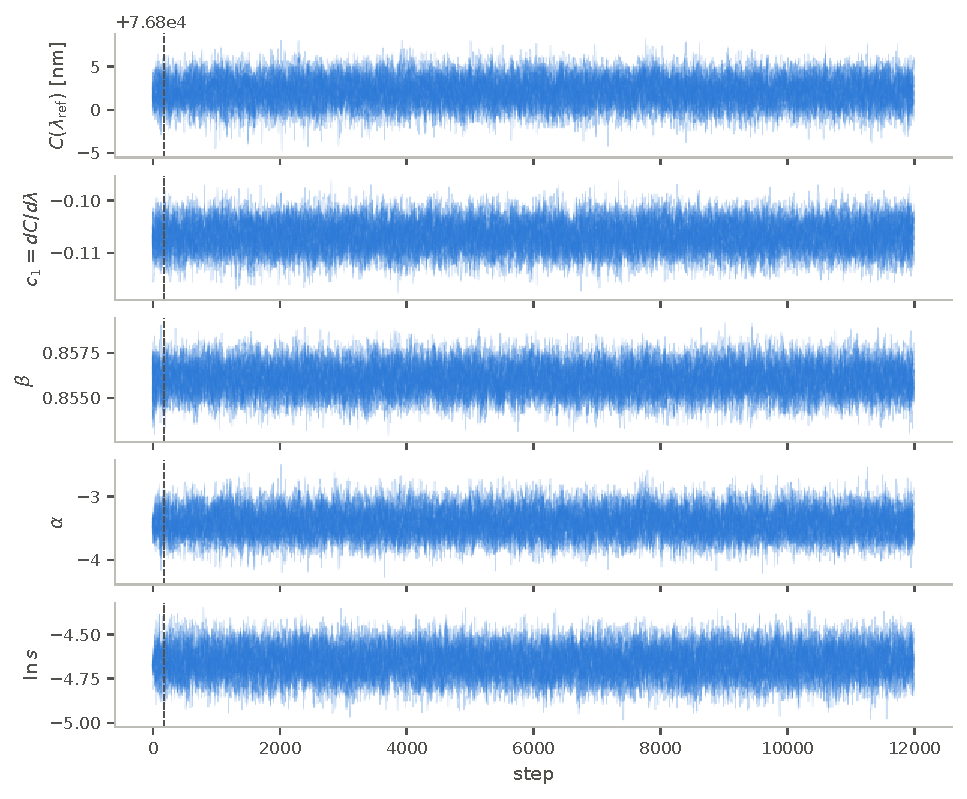
\includegraphics[width=\textwidth]{chains_SPIRou.pdf}
\caption{SPIRou walkers. The dashed line marks the end of the burn-in.}
\end{figure}

\begin{figure}[h]
\centering
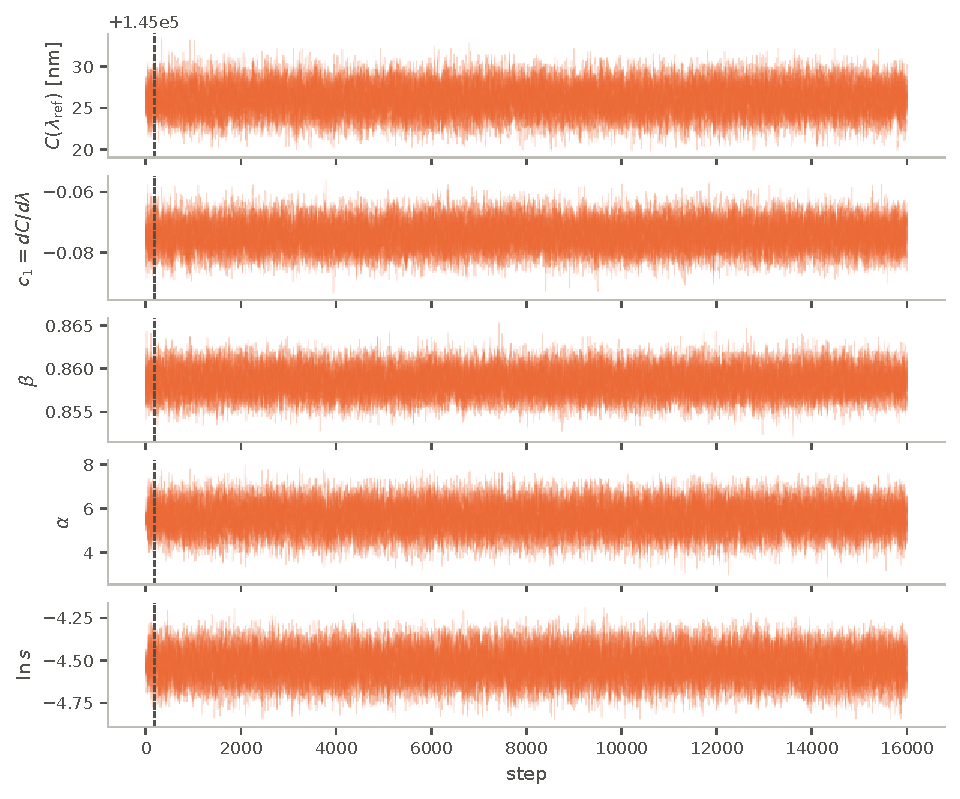
\includegraphics[width=\textwidth]{chains_NIRPS.pdf}
\caption{NIRPS walkers. The dashed line marks the end of the burn-in.}
\end{figure}

\begin{figure}[h]
\centering
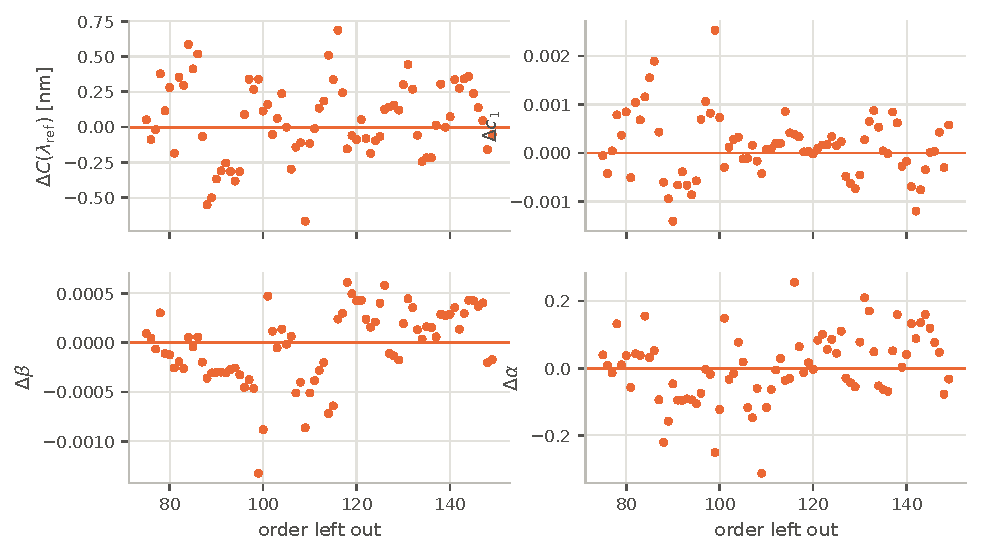
\includegraphics[width=\textwidth]{jackknife_NIRPS.pdf}
\caption{NIRPS jackknife, as in Figure~\ref{fig:jacksp}.}
\end{figure}

\begin{figure}[h]
\centering
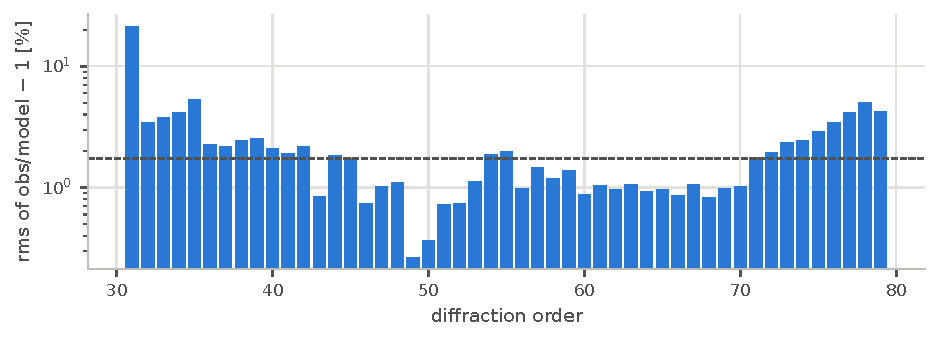
\includegraphics[width=\textwidth]{per_order_SPIRou.pdf}\\
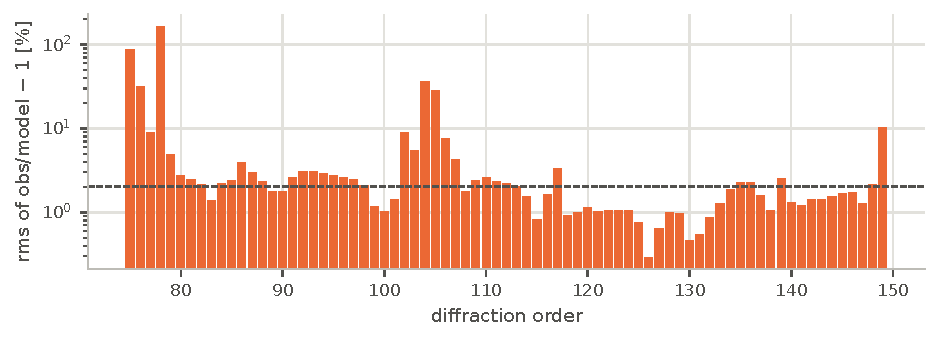
\includegraphics[width=\textwidth]{per_order_NIRPS.pdf}
\caption{Rms of the relative residual in each order, SPIRou (top) and NIRPS (bottom). The dashed line is the median over orders.}
\end{figure}

\begin{figure}[h]
\centering
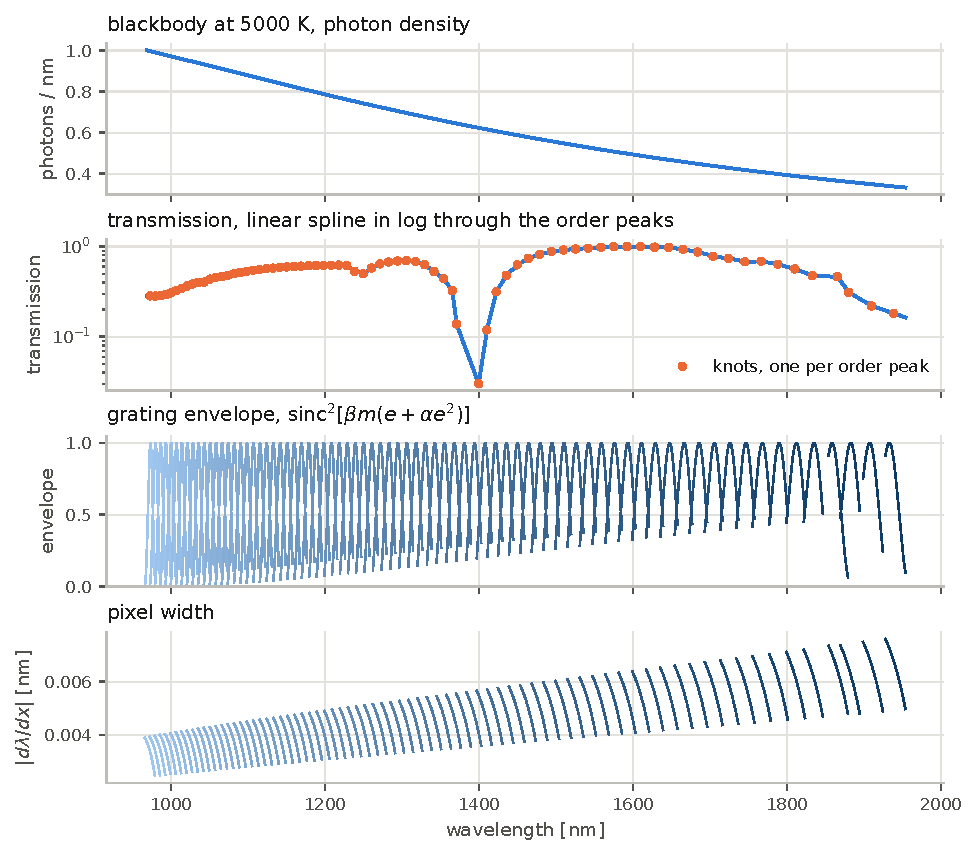
\includegraphics[width=\textwidth]{components_NIRPS.pdf}
\caption{The four terms of the NIRPS model.}
\end{figure}

\begin{figure}[h]
\centering
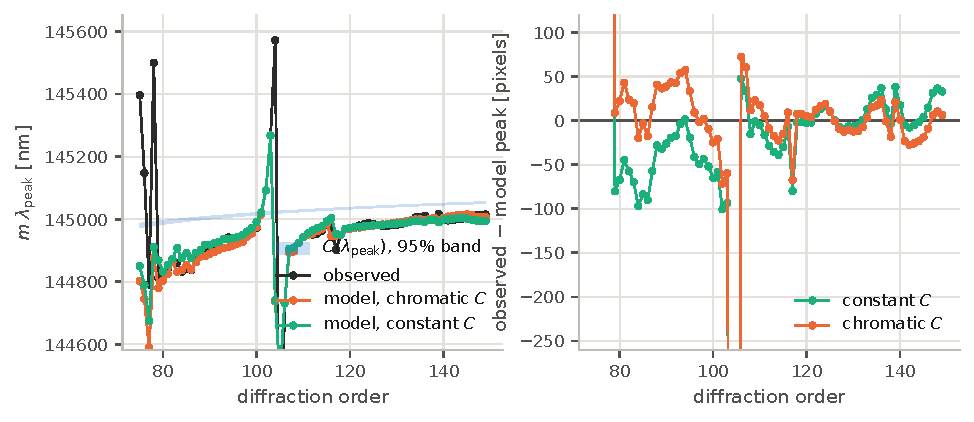
\includegraphics[width=\textwidth]{peaks_NIRPS.pdf}
\caption{NIRPS peak positions, as in Figure~\ref{fig:peaks}.}
\end{figure}

\begin{figure}[h]
\centering
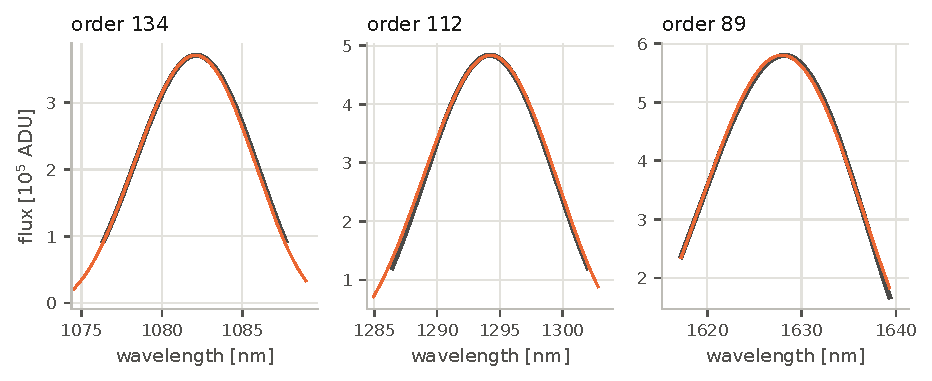
\includegraphics[width=\textwidth]{zoom_NIRPS.pdf}
\caption{Three NIRPS orders at full scale.}
\end{figure}

\clearpage
%======================================================================
\section{Program output}
\label{app:logs}

\subsection{\code{mkblaze.py}, SPIRou}
{\scriptsize
\VerbatimInput{mkblaze_log.txt}
}

\subsection{\code{fit\_blaze.py}, SPIRou}
{\scriptsize
\VerbatimInput{fitlog_SPIRou.txt}
}

\subsection{\code{fit\_blaze.py}, NIRPS}
{\scriptsize
\VerbatimInput{fitlog_NIRPS.txt}
}

%======================================================================
\section{Reproducing this report}
\label{app:repro}

Every number in this report is a macro written by \code{report/make\_numbers.py}, and every figure is drawn by \code{report/make\_report\_figures.py}. Both read the results of \code{report/run\_analysis.py} (order identification, fit, MCMC, jackknife, profiles) and \code{report/run\_comparison.py} (model comparison). From the top of the repository, the command
\begin{verbatim}
python characterize.py
\end{verbatim}
runs the whole chain and compiles this document. \verb|python characterize.py --no-report| runs the analysis only, and \verb|--report-only| rebuilds the figures and this document from existing results. The best-fit model and its parameters are stored in \code{blaze\_model.fits}: the header holds \code{MODCA0}, \code{MODCA1}, \code{MODBETA}, \code{MODASYM}, \code{MODTEFF}, \code{MODWMAX} and \code{MODORD0}, and the \code{TRANS\_KNOTS} extension holds the spline knots.

\end{document}
